\section{Machine Learning}

\begin{itemize}
\item What is machine learning?

\item Why is it useful for HEP? (Problems are multivariate...)

\item Supervised learning, i.e.\ have labelled data.

\item Binary classification tasks: Every training example has a label indicating
  the class membership.

\item In HEP, the positive class is typically referred to as \emph{signal} while
  the negative class is referred to as \emph{background}.

\item What is training data, etc.

\item What is training.

\item Overfitting?
\end{itemize}


\subsection{Boosted Decision Trees}

Boosted decision trees (BDT) are classification and regression algorithms
composed of multiple \emph{decision trees}. This ensemble of decision trees is
created using an algorithm referred to as \emph{boosting}, which iteratively
fits shallow decision trees--or in general, any \emph{weak learning
  algorithm}--to altered versions of the training data. The training data is
modified at every iteration to emphasise errors made in previous
iterations. Finally, the predictions of the ensemble of trees are combined with
the goal of providing superior classification/regression performance compared to
a single decision tree. In the following a description of one of the BDT
algorithms implemented in \textsc{TMVA}~\cite{TMVA} is given, which is later
used in the search for Higgs boson pair production.


\subsubsection{Classification and Regression Trees}

Classification and regression trees~\cite{Breiman:1984jka,hastie09}, hereafter
collectively referred to as \emph{decision trees}, are used as the basis for
BDT. A decision tree partitions an $n$-dimensional space with coordinates
$\myvec{x} = (x_1, \dots, x_n)$ by recursively performing binary splits along
the coordinate axes until a stopping criterion is met. The resulting binary tree
structure and partitioning is illustrated in \Cref{fig:decision_tree} for a
two-dimensional example. A decision tree with $J$~leaf nodes partitions the
input space into $J$~mutually disjoint subregions denoted by $R_j$ for
$j = 1, \dots, J$. A constant value $c_j$ is assigned to every region $R_j$ such
that the prediction of a decision tree for a point~$\myvec{x}$ can expressed as
\begin{align*}
  h\bigl( \myvec{x}; \{c_j, R_j\}_{j=1}^{J} \bigr) = \sum_{j = 1}^{J} c_j \, \mathbf{1}(\myvec{x} \in R_j) \qquad \text{with} \qquad \mathbf{1}(\myvec{x} \in R_j) =
  \begin{cases}
    1, & \myvec{x} \in R_j \\
    0, & \text{else}
  \end{cases} \,\text{,}
\end{align*}
where $\{c_j, R_j\}_{j=1}^{J}$ fully specifies the decision
tree~\cite{hastie09}.

\begin{figure}[htbp]
  \centering

  \begin{subfigure}[b]{0.46\textwidth}
    \centering
    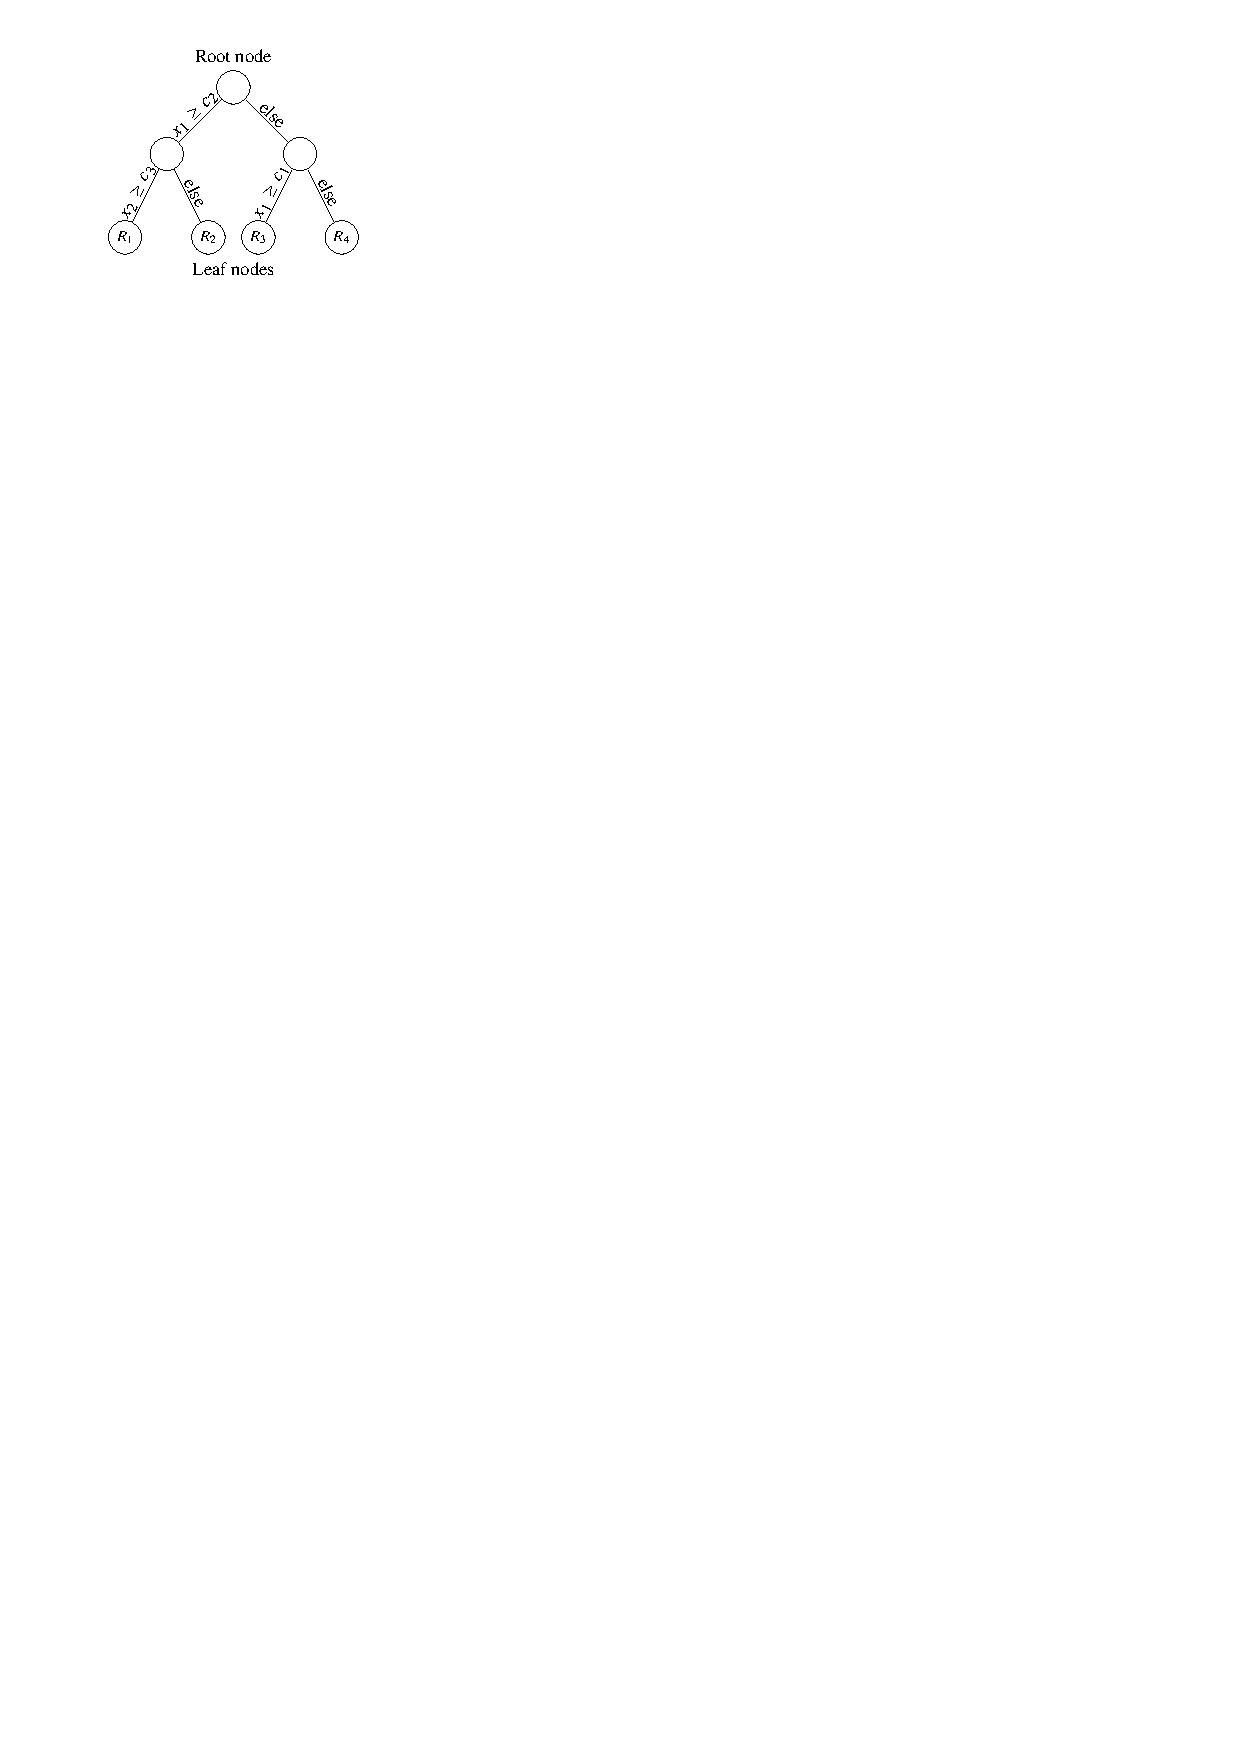
\includegraphics[scale=1.05]{ml/decision_tree}
    \caption{Binary tree structure of a decision tree.}
  \end{subfigure}\hfill%
  \begin{subfigure}[b]{0.46\textwidth}
    \centering
    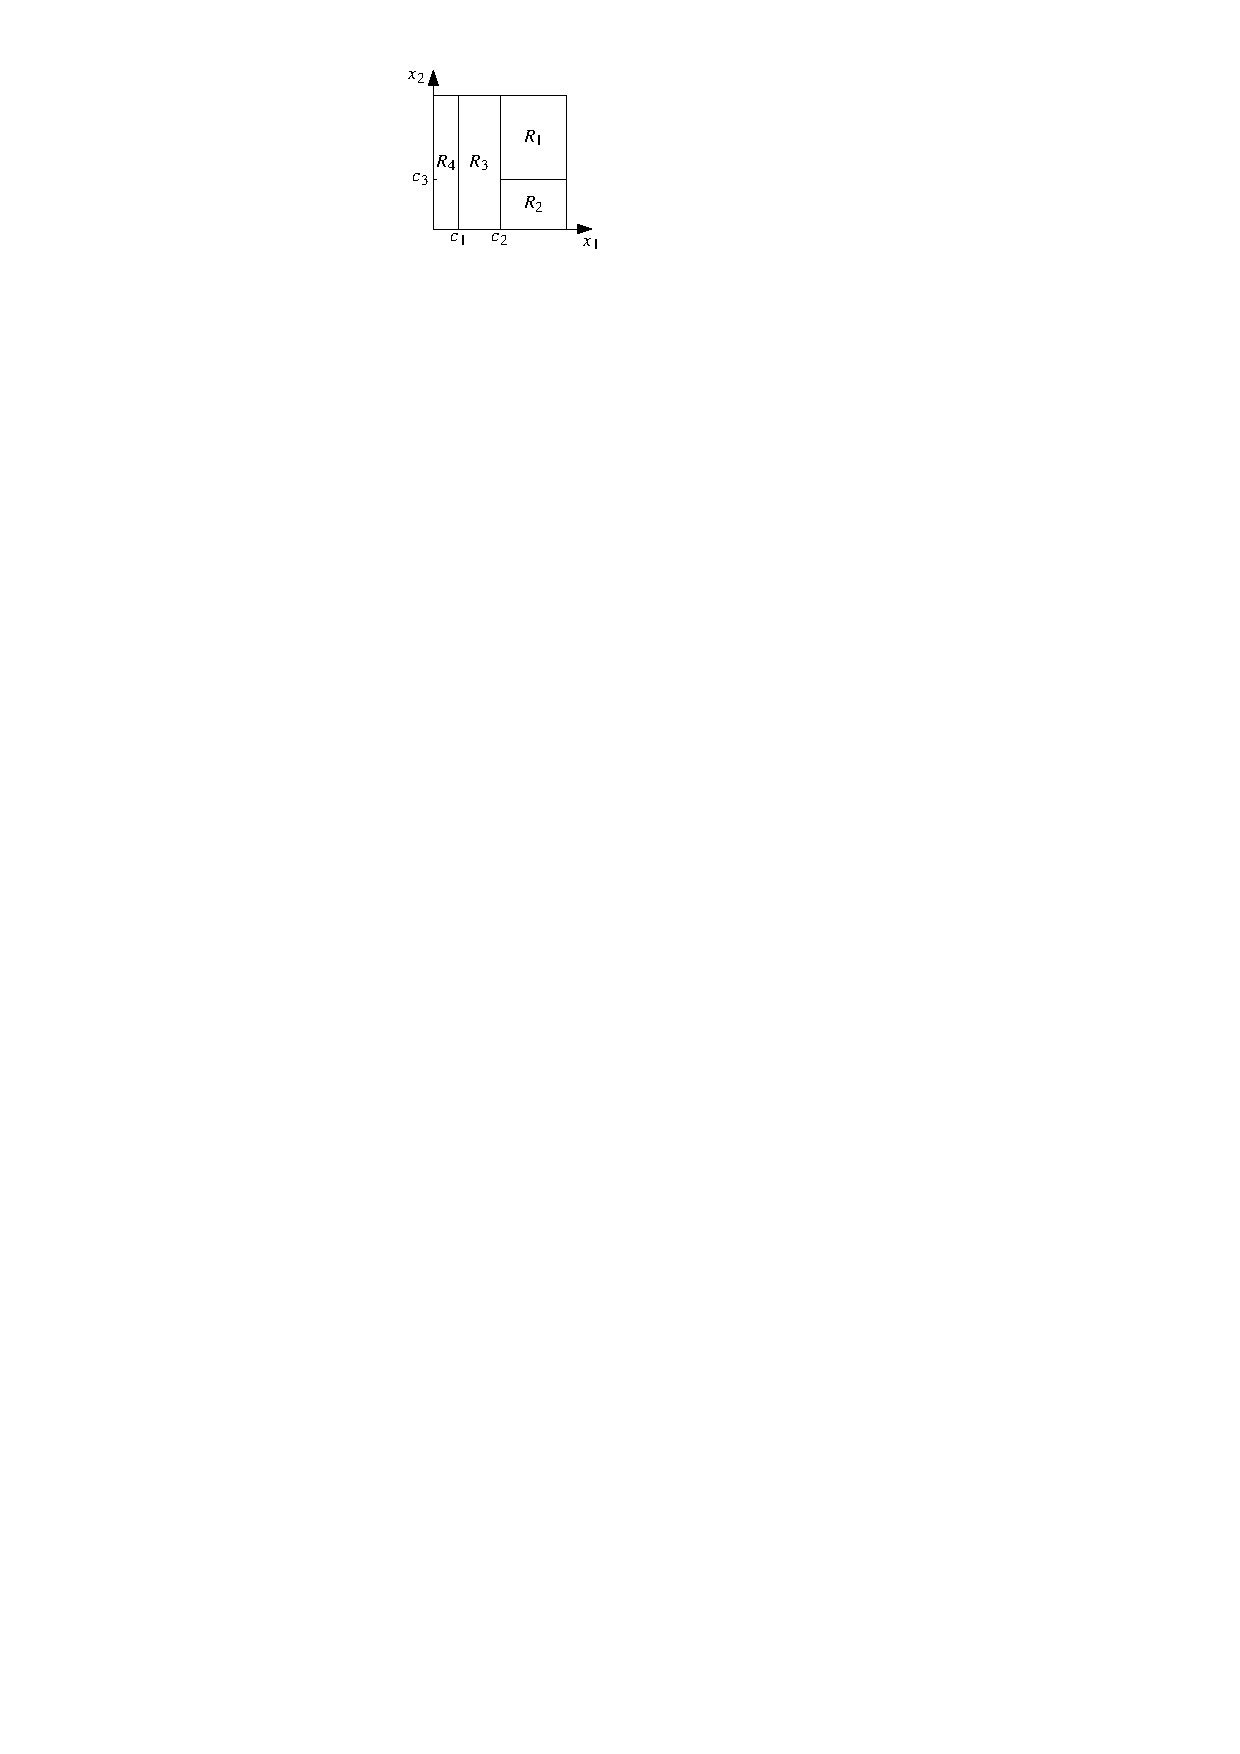
\includegraphics[scale=1.05]{ml/decision_tree_partitioning}
    \vspace*{0.7em}
    \caption{Partitioning resulting from the binary tree in (a).}
  \end{subfigure}\hfill%

  \caption{Example of a decision tree operating on a two-dimensional space with
    coordinates $\myvec{x} = (x_1, x_2)$. The tree has a depth of two and four
    leaf nodes that define the regions $R_1, \dots, R_4$. The figure is adapted
    from Ref.~\cite{hastie09}.}%
  \label{fig:decision_tree}
\end{figure}

Classification trees are constructed with the goal that the partitioning of the
input space yields subregions with low impurity, that is, the regions are mostly
populated by training examples of a single class. In this case, the impurity of
a tree node is quantified by the Gini index
\begin{align*}
  I_{\text{G}}(p) = 2 p (1 - p) \,\text{,}
\end{align*}
where $p$ is the proportion of examples from the positive class in a given
node~\cite{hastie09}. A \emph{greedy} strategy is adopted to grow decision trees
by performing the best possible split at every node. This split is determined by
minimising the weighted sum of Gini impurities of the resulting daughter nodes,
where impurities are weighted according to the total weight of training examples
populating a given node. In the classification case, the constants $c_j$
assigned to leaf nodes of the tree are either--depending on the algorithm
configuration--the proportion of examples from the positive class or the class
label of the majority class in a given leaf node.

Regression trees are constructed using a similar approach, however, with an
altered splitting criterion and different assigment of constants to leaf
nodes. Consider the split of a parent node into a left (L) and right (R)
daughter node. Let $(y, w)$ denote the tuple of regression target and weight of
a given training example. Moreover, let $T_{\text{L}}$ and $T_{\text{R}}$ denote
the set of $(y, w)$ for training examples populating the left and right daughter
node, respectively. The constants $c_{\text{L}}$ and $c_{\text{R}}$ assigned to
the daughter nodes are given by
\begin{align*}
  c_{\text{L}} = \frac{\sum_{(y, w) \in T_{\text{L}}} w y}{\sum_{(y, w) \in T_{\text{L}}} w} \qquad \text{and} \qquad c_{\text{R}} = \frac{\sum_{(y, w) \in T_{\text{R}}} w y}{\sum_{(y, w) \in T_{\text{R}}} w} \,\text{,}
\end{align*}
which is the weighted mean of the regression target for the training examples
populating the left and right node, respectively. The best possible split of a
node in a regression tree is chosen such that the squared error defined as
\begin{align*}
  \sum_{(y, w) \in T_{\text{L}}} w (y - c_{\text{L}})^2 + \sum_{(y, w) \in T_{\text{R}} } w (y - c_{\text{R}})^2
\end{align*}
is minimised.


\subsubsection{Boosting of Decision Trees}

Boosting is an approach of solving predictions tasks by constructing additive
models of the form
\begin{align*}
  F_{M}\bigl(\myvec{x}; \{ \beta_m, \gamma_{m} \}_{m=1}^{M} \bigr) = \sum_{m = 1}^{M} \beta_m b(\myvec{x}; \gamma_{m}) \,\text{,}
\end{align*}
where $\beta_m$ are coefficients and $b(\myvec{x}; \gamma_{m})$ are basis
functions parameterised
by~$\gamma_{m}$~\cite{Friedman:2000,Friedman:2001wbq}. While there is some
flexibility in choosing the family of basis functions, boosting is typically
applied to decision trees.
% Given a sample of training data, the model is fit using an
% iterative procedure in which the $m$-th stage of the model, which is given by
% \begin{align*}
%   F_{m}\bigl(\myvec{x}; \{ \beta_{n}, \gamma_{n} \}_{n=1}^{m} \bigr) = F_{m - 1}\bigl( \myvec{x}; \{ \beta_{n}, \gamma_{n} \}_{n=1}^{m-1} \bigr) + \beta_m b(\myvec{x}; \gamma_{m}) \,\text{,}
% \end{align*}
% is determined by choosing $\beta_{m}$ and $\gamma_{m}$ such that an objective
% function is improved~\cite{hastie09}. Notably, the $m$-th stage does not alter
% the parameters~$\{ \beta_{n}, \gamma_{n} \}_{n=1}^{m-1}$.
The following is concerned with a boosting algorithm referred to as
\emph{gradient boosting}~\cite{Friedman:2001wbq}. Gradient boosting is an
algorithm for constructing additive models that minimise arbitrary
differentiable loss functions, thus making it a useful tool for solving various
prediction tasks.

Consider a binary classification problem with predictors~$\myvec{X}$ and class
labels~$Y$, which are $Y = +1$ for the positive and $Y = -1$ for the negative
class. Both $\myvec{X}$ and $Y$ are random variables. Further, let
\begin{align}
  L(Y, F(\myvec{X})) = \log\mathopen{}\left(
  1 + e^{-Y F(\myvec{X})}
  \right)\mathclose{}
  \label{eq:loss_gradboost}
\end{align}
be a loss function and $F$~a function of the predictors. The function that
minimises the expected loss is given by
\begin{align*}
  F^{*\!}(\myvec{x})
  = \argmin_F \, \expect[ L(Y, F) \mid \myvec{X} = \myvec{x} ]
  = \log\mathopen{}\left(
  \frac{
  \mathbb{P}(Y = +1 \mid \myvec{X} = \myvec{x})
  }{
  \mathbb{P}(Y = -1 \mid \myvec{X} = \myvec{x})
  }
  \right)\mathclose{} \,\text{,}
  %\label{eq:gradboost_logodds}
\end{align*}
which are the conditional log-odds of an observation with predictors~$\myvec{x}$
belonging to the positive class~\cite{Friedman:2000}. Knowledge of $F^{*\!}$
would solve the classification task since
\begin{align}
  \mathbb{P}(Y = +1 \mid \myvec{X} = \myvec{x}) = \frac{1}{1 + e^{-F^{*\!}(\myvec{x})}}
  \qquad \text{and} \qquad
  \mathbb{P}(Y = -1 \mid \myvec{X} = \myvec{x}) = \frac{1}{1 + e^{+F^{*\!}(\myvec{x})}} \,\text{,}
  \label{eq:gradboost_probas}
\end{align}
thus motivating the choice of loss function in \Cref{eq:loss_gradboost} for
binary classification.

% Gradient boosting can be used to find an additive model that minimises this
% loss function for a finite sample,

% with this loss function can be used to
% find an approximation to $F^{*\!}(\myvec{x})$

% with decision trees can be used to find an approximation to
% $F^{*\!}(\myvec{x})$ using a finite sample of training data.

An algorithm referred to as \textsc{TreeBoost} proposed by
Friedman~\cite{Friedman:2001wbq} is outlined. \textsc{TreeBoost} uses gradient
boosted decision trees and the loss function in \Cref{eq:loss_gradboost} to fit
a binary classifier to a sample of training data. A version of this algorithm is
employed in \textsc{TMVA}~\cite{TMVA}, which provides the BDT implementation
used in this thesis. The description is based on Ref.~\cite{Friedman:2001wbq}
with some modifications (e.g.\ allowing training data to be weighted).

\vspace{11pt}
\noindent\textbf{\textsc{TreeBoost} algorithm for binary classification} \\[11pt]
\noindent Inputs:
\begin{itemize}[itemsep=1pt,topsep=4pt]
\item Training data $\{(\myvec{x}_i, y_i, w_i)\}_{i = 1}^{N}$ with
  predictors~$\myvec{x}_i$, class labels $y_i$, and weights~$w_i$.
\item Number of boosting iterations $M$.
\item Shrinkage parameter~$\nu$ ($0 < \nu \leq 1$).
\item Hyperparameters of the regression tree algorithm.
\end{itemize}

\vspace{6pt}
\noindent Algorithm:
\begin{enumerate}[itemsep=1pt,topsep=4pt]

\item The model is initialised to predict a constant given by
  \begin{align*}
    F_0(\myvec{x}) = \log\mathopen{}\left( \frac{1 + \bar{y}}{1 - \bar{y}}
    \right)\mathclose{}
    \qquad \text{with} \qquad
    \bar{y} = \frac{\sum_{i=1}^{N} w_i y_i}{\sum_{i=1}^{N} w_i} \,\text{,}
  \end{align*}
  which are the (unconditional) log-odds of $Y = +1$ estimated using the
  training data.

\item For $m = 1$ to $M$:
  \begin{enumerate}[itemsep=1pt]

  \item Calculate the pseudoresiduals
    \begin{align*}
      r_i
      = - \left. \frac{\partial L(y_i, F(\myvec{x}_i))}
      {\partial F(\myvec{x}_i)}\right|_{F(\myvec{x}_i) = F_{m - 1}(\myvec{x}_i)}
      \overset{\text{Eq.\ (\ref{eq:loss_gradboost})}}{=}
      \frac{y_i}{1 + \exp(y_i F_{m-1}(\myvec{x}_i))}
    \end{align*}
    for all training examples.
    % , where $\myvec{x}_i$ are the predictors and $y_i$ the class label of the
    % $i$-th training example, respectively.

  \item Fit a regression tree to the training data to estimate the
    pseudoresiduals using the predictors~$\myvec{x}$. The prediction of the
    fitted regression tree is denoted by
    $h\bigl( \myvec{x}; \{c_{jm}, R_{jm}\}_{j=1}^{J_{m}} \bigr)$, where $J_{m}$
    is the number of leaf nodes, $c_{jm}$ is the constant predicted by the
    $j$-th leaf node, and $R_{jm}$ is the region defined by the $j$-th leaf
    node.

  \item The leaf node constants of the regression tree,
    $\{c_{jm}\}_{j=1}^{J_{m}}$, are updated to minimise
    \begin{align*}
      \sum_i w_i \cdot
      L\mathopen{}\left( y_i, F_{m - 1}(\myvec{x}_i)
      + h\bigl( \myvec{x}_i; \{c_{jm}, R_{jm}\}_{j=1}^{J_{m}} \bigr)
      \right)\mathclose{}
      \,\text{,}
    \end{align*}
    where the sum goes over all training data. This optimisation problem has no
    analytical minimiser for the loss function in
    \Cref{eq:loss_gradboost}. Instead, the $\{c_{jm}\}_{j=1}^{J_{m}}$ are chosen
    to approximately minimise the above criterion by performing a single step of
    Newton's method.\footnote{The starting point for Newton's method is taken to
      be $c_{jm} = 0$ for all leaf nodes.} This yields the updated leaf node
    constants
    \begin{align*}
      c_{jm}^\prime = \frac{ \sum_i w_i r_i }{ \sum_i w_i |r_i| (1 - |r_i|)} \,\text{,}
    \end{align*}
    where the sum goes over the training data populating the $j$-th leaf node of
    the tree. This step is specific to the \textsc{TreeBoost} algorithm by
    Friedman.

  \item Determine the $m$-th stage of the model by setting
    \begin{align*}
      F_m(\myvec{x}) = F_{m - 1}(\myvec{x})
      + \nu \cdot h\bigl( \myvec{x}; \{c_{jm}^\prime, R_{jm}\}_{j=1}^{J_{m}} \bigr)
      \,\text{,}
    \end{align*}
    where $\nu$ is a parameter of the boosting algorithm referred to as the
    \emph{shrinkage} or \emph{learning rate}. Generally, the shrinkage is set to
    values below unity such that every stage of boosting performs a suboptimal
    update. This serves as a form of regularisation to prevent overfitting.

  \end{enumerate}

\item The final prediction of the boosting procedure,
  $F_{M\hspace{-0.07em}}(x)$, can be used to estimate the probability
  $\mathbb{P}(Y = +1 \mid \myvec{X} = \myvec{x})$ according to
  \Cref{eq:gradboost_probas} as
  \begin{align*}
    p(\myvec{x}) = \frac{1}{1 + e^{-F_{M\hspace{-0.07em}}(\myvec{x})}} \,\text{.}
  \end{align*}
  In HEP, this quantity is commonly referred to as the \emph{BDT score}.

\end{enumerate}
\vspace{8pt} This algorithm is reminiscent of the classical gradient descent
algorithm for optimisation, however, in the case of gradient boosting the
optimisation is performed in the space of
functions~\cite{Friedman:2001wbq}. Steps 2a) and 2b) of the algorithm serve to
estimate the negative gradient of the loss function with respect to
$F(\myvec{x})$, which is evaluated at the function estimate of the previous
boosting iteration. In gradient descent, the step size of the update is often
determined by performing a line search along the direction of steepest
descent. This is the task of step 2c) in which the step size is determined,
however, for \textsc{TreeBoost} the size of the gradient descent step is
determined on a per-leaf basis. Finally, 2d) performs the (intentionally
suboptimal) gradient descent update.


\subsection{Neural Networks}%
\label{sec:neural_networks}

\subsubsection{Recurrent Neural Networks}%
\label{sec:rnn}


%%% Local Variables:
%%% mode: latex
%%% TeX-master: "../../phd_thesis"
%%% End:
